\documentclass[12pt, dvipsnames, oneside, a4paper, titlepage, usenames]{report}
% Report => longer text containing several chapters like a book, thesis etc.
% Using direclty 'book' would create mess in positioning of page numbers.

\usepackage[utf8]{inputenc} % Input encoding - without this non-ascii symbols get totally screwed
\usepackage[T1]{fontenc} % Font encoding - without this non-ascii symbols are created "in an amateur way"
\usepackage{mathpazo} % Palatino Linotype with math
\usepackage{courier} % Courier fonts
\usepackage{yfonts} % Schwabacher
\usepackage{anyfontsize} % Custom font sizes
\usepackage[top=2.5 cm, left=2.5cm, right=2.5cm]{geometry} % Margins
\usepackage{xparse} % Enhanced custom commands arguments parsing
\usepackage{textcomp} % Straight quotes (not apostrophes)
\usepackage{makeidx} % Creating index
\usepackage{hyperref} % Hyperlinks
\usepackage[dvipsnames]{xcolor} % Colors
\usepackage{caption} % Captions magic
\usepackage{verbatim} % Comments
\usepackage{listings} % Code blocks
\usepackage{graphicx} % Inserting pictures
\usepackage{tikz}
\usetikzlibrary{tikzmark}

\sloppy % Prevents line overflowing

% Page number height adjustment
%\setlength{\footskip}{45pt}
% WARNING! The higher the set number is the LOWER the page number is placed!

% Links color setup, it's {R G B} with floats from 0 to 1, non-bordering values don't contain zero (e.g., '.5')
\hypersetup{
    linkbordercolor={1 0 0},
    urlbordercolor={0 0 1}
}

% Code listings global settings
\lstset{
    alsoletter={/"},
    basicstyle=\fontsize{10.5}{\baselineskip}\selectfont\ttfamily,
    breakindent=0pt,
    breaklines=true,
    breakatwhitespace=true,
    escapeinside={(*}{*)},
    frame=single,
    gobble=8,
    postbreak=\mbox{\textcolor{red}{$\hookrightarrow$}},
    rulecolor=\color{black},
    showstringspaces=false,
    upquote = true
}

% Java code listings settings
\lstdefinelanguage{Java}{
    commentstyle=\color{ForestGreen},
    keywordstyle=\color{blue},
    stringstyle=\color{ForestGreen},
    morekeywords={class,public,private,protected,static,this},
    morestring=[b]"
}

% XML code listings settings
\lstdefinelanguage{XML}{
    alsoletter={:},
    commentstyle=\color{gray},
    keywordstyle=\color{blue},
    stringstyle=\color{ForestGreen},
    morecomment=[s]{<?}{?>},
    morekeywords={class,id,ref,xmlns,xmlns:context,xsi},
    morestring=[b]"
}

\newcommand{\newchapter}[1]{\chapter*{#1}\addcontentsline{toc}{chapter}{#1}}

\newcommand{\newsection}[1]{\section*{#1}\addcontentsline{toc}{section}{#1}}

\newcommand{\newsubsection}[1]{\subsection*{#1}\addcontentsline{toc}{subsection}{#1}}

\newcommand{\highlight}[2]{\vspace{\baselineskip}\noindent\textcolor{#2}{\textbf{#1}}}

\newcommand{\warning}{\highlight{WARNING! }{red}}

\newcommand{\note}{\highlight{NOTE: }{ForestGreen}}

\newcommand{\todo}{\highlight{TODO }{blue}}

\newcommand{\example}{\highlight{Example: }{black}}

\newcommand{\textbfcolor}[2]{\textcolor{#1}{\textbf{#2}}}

\NewDocumentCommand{\tikzmarknodebf}{m m O{black}}{\tikzmarknode{#1}{\textbfcolor{#3}{#2}}}

\NewDocumentCommand{\drawarrow}{m m O{black} O{.3} O{}}{\draw[stealth-stealth,line width=.6mm,shorten <=2pt,shorten >=2pt,#3,opacity=#4] (#1) to[#5] (#2);}

\makeindex

\begin{document}
    \hyphenation{abbre-vi-a-tion acti-vely adleman although ambi-gu-ous another assign assigns assig-ning assign-ment autho-rity beside decryp-tion default defi-ned demands diffe-rent dis-co-ve-ring divi-sible ena-bling encap-su-alte encap-su-la-ting encap-su-la-ton encrypt encryp-ting eve-ry-where exam-ple exe-cu-tion focu-ses gene-rally human impe-ra-tive inco-ming instal-led instruc-ti-ons itself keep keeping machine mana-ge-ment methods oracle rea-so-na-ble remote return rivest shamir tera-byte tera-bytes trans-for-ming without}

    \begin{titlepage}
        \vspace*{\fill}
        \begin{center}
            {\swabfamily\fontsize{90}{90}\selectfont Gro{\ss}buch\par}
            \vspace{1cm}
            \mbox{{\fontsize{20}{20}\selectfont A need--to--know for Java developers}}
            \vspace{3cm}
        \end{center}
        \vspace*{\fill}
        \begin{flushright}
            Petr Machovec
        \end{flushright}
    \end{titlepage}

    \tableofcontents

    \newchapter{General Knowledge}

    \newsection{Object--Oriented Programming}
    \index{Object--oriented programming}
    \label{objectorientedprogramming}
    It's a programming paradigm in which data are encapsulated into objects together with tools for manipulating these data. An object holds data in fields (also called attributes) and provides methods (also called functions) for manipulating with these data (typically from other objects). Java and~most other languages using the~object paradigm like C\# or C++ are~not~pure object languages, because they contain primitive data types like \textit{int} or \textit{boolean}. In~pure object languages all~data (each variable) must be object. An~example of a~pure object language is Smalltalk (and~there is~probably no~other).

    \warning Object--oriented programming is~not contradictory to~\hyperref[imperativeprogramming]{imperative programming} (or~even \hyperref[declarativeprogramming]{declarative programming}, see further).

    \newsection{Basic Concepts of Object--Oriented Programming}

    \newsubsection{Encapsulation}
    \index{Encapsulation}

    \newsubsection{Inheritance}
    \index{Inheritance}

    \newsubsection{Polymorphism}
    \index{Polymorphism}

    \newsubsection{Abstraction}
    \index{Abstraction}

    \newsection{Object VS Data Structure}

    \newsection{Object--Oriented VS Procedural Programming}
    \index{Procedural programming}

    \newsection{Imperative Programming}
    \index{Imperative programming}
    \label{imperativeprogramming}
    It's a~programming paradigm in which a~program behavior is changed by~specified statements. It's opposite of~\hyperref[declarativeprogramming]{declarative programming}.

    \warning It is \textbf{not} contradictory to \hyperref[objectorientedprogramming]{object--oriented programming}, imperative languages can be object--oriented. Actually, today's most used object--oriented languages (Java, C\#, C++) are imperative.

    \newsection{Declarative Programming}
    \index{Declarative programming}
    \label{declarativeprogramming}
    It's a~programming paradigm in which programs describe their desired results without explicitly listing commands or steps that must be performed. It's opposite~of~\hyperref[imperativeprogramming]{imperative programming}. Typical examples of~declarative languages are~SQL or~Prolog. Oracle's PL/SQL is a~kind of~hybrid language using imperative statements combined with declarative SQL. Even declarative languages can be \hyperref[objectorientedprogramming]{object--oriented} (there~is an~object extension for~Prolog).

    \newsection{Compiled VS Interpreted Languages}
    \index{Compiled language}
    \index{Interpreted language}

    \newsection{Variable VS Field VS Property}
    \index{Variable}
    \index{Field}
    \index{Property}
    \label{variablefieldproperty}
    \begin{itemize}
        \item \textbf{Variable} is a~general term denoting data with named identifier.
        \item \textbf{Field} is a~variable defined in~a~class outside any~method. Fields store parts of~class instance states. Class constants are~fields, variables defined inside \mbox{methods/functions} and~cycles are~not.
        \item \textbf{Property} is a~field that is~exposed to~outside of~the~class, typically by~getters and~setters.
    \end{itemize}

   \section*{\fontsize{17}{17} \selectfont Application VS Process VS Program VS Service VS Thread}
   \addcontentsline{toc}{section}{Application VS Process VS Program VS Service VS Thread}
   \index{Application}
   \index{Process}
   \index{Program}
   \index{Service}
   \index{Thread}
   \index{Computer program}
   \label{applicationprocessprogramservicethread}
   \begin{itemize}
        \item \textbf{Program} is the~most general term of these. It's included in all others. A~computer program is a~set of~instructions that can be executed on a~computer.
        \item \textbf{Application} is a~computer program with which, when it's executed, users actively interact.
        \item \textbf{Process} is a~particular executed and~running instance of a~program.
        \item \textbf{Service} is a~process that runs continuously in the~background without active interaction with a~user. I.e., it's the opposite of application.
        \item \textbf{Thread} is a~set of consecutive steps performed one by~one in a~process. A~process can be separated to~more threads which can run in~parallel (if~the~program implementation supports~it).
    \end{itemize}

    \newsubsection{Web Servive}
    \index{Web service}
    \label{webservice}
    It's any~program executed or~continuously running on a~remote computer, with which programs on~other computers communicate over the~\hyperref[internetweb]{Web}, i.e.,~using the~\hyperref[http]{HTTP} protocol. A~program called \hyperref[clientserverarchitecture]{client}, running on a~user's computer, sends a~request to~another~program called \hyperref[clientserverarchitecture]{server} running on~the~remote computer (the~same computer as the~target remote program), the~server delegates the~request to~the~remote program, the~remote program prosesses the~request and~sends a~response to~the~server, which then delegates it back to~the~client.

    \warning The~term \textit{web service} is~ambiguous. Sometimes it denotes solely the~remote program, sometimes it includes even the~server. Also, opposite to~a~standard \hyperref[applicationprocessprogramservicethread]{service} the~remote program doesn't have to run continuously. Only the~server does.

    \newsection{32b VS 64b}
    \index{32b}
    \index{64b}
    \label{32bvs64b}

    \newsection{Distributed System}
    \index{Distributed system}
    \label{distributedsystem}
    It's a~system whose components are~located on~different networked computers, which communicate and~coordinate their actions by~passing messages to~one~another. All~components communicate to~achieve a~common goal. Distributed systems have three main characteristics:
    \begin{itemize}
        \item Components work \hyperref[concurrency]{concurrently}.
        \item There is no global clock\,--\,no~time synchronization among components.
        \item Components fail independently\,--\,if~one~component fails, other components are~not~affected.
    \end{itemize}
    \noindent Examples are~computer networks (including the~\hyperref[internetweb]{Internet}) or~telephone networks.

    \newsubsection{Distributed Version Control System}
    \index{Distributed version control system}
    \label{distributedversioncontrolsystem}
    It's~a~version control system where each user owns a~copy (mirror) of~the~whole code base including the~whole history. The~typical example of~such system is~\hyperref[git]{Git}.

    \newsection{Multitasking}
    \index{Multitasking}

    \newsection{Concurrency}
    \index{Concurrency}
    \label{concurrency}

    \newsection{Loose Coupling VS Tight Coupling}
    \index{Loose coupling}
    \index{tightcoupling}
    \label{loosetightcoupling}

    \newsection{Base64}
    \index{Base64}
    \label{base64}
    It's an~encoding used for~representation of~any array of~bytes as an~ASCII string. The~name refers to the~size of~the~set of~resulting characters, which is~64. It~encodes always three bytes to~four characters. If~the~length of~the~input byte array is~not~divisible by~three, one or~two special bytes are~added to~its~end. This results in~one or~two equals signs at~the~end of~the~resulting string.

    \newsection{Null Design Pattern}
    \index{Null design pattern}


    \newchapter{Java Basics}

    \newsection{Bytecode}
    \index{Bytecode}
    \label{bytecode}
    Bytecode is the result of compilation of Java code. It's stored in \textit{.class} files. For~people it's an unreadable mess (it's a type of \hyperref[bytecodebinarycode]{binary code}), however it isn't the machine code which a processor can read. It must be read and further transformed to the machine code by JVM, i.e.,~it's a~middle step between written Java code and its execution. The reason of this approach is that bytecode is transferable between platforms (that's why sometimes it's called \textit{portable code})\,--\,no~matter on what platform (platform\,=\,OS\,+\,hardware, hardware\,=\,\hyperref[32bvs64b]{32b~VS~64b}) the original Java code was written and compiled, the resulting bytecode will be executable on any other platform. The~thing which is different for each platform is \hyperref[jdkjrejvm]{JRE}.

    For comparison consider C++. In this programming language the result of compilation is directly the machine code, which must be different for each platform, i.e.,~the thing in C++ which is different for each platform is the compiler.

    By the way the approach with millde--step code is used also by C\#, which is compiled to~so~called CIL (Common Intermediate Language). The~main difference of CIL from bytecode is that CIL is human--readable, although it's quite complicated (and~useless).

    \newsubsection{Bytecode VS Binary Code}
    \index{Binary code}
    \label{bytecodebinarycode}
    Binary code is generally any code in a~form readable for a~computer. It can be machine code read by processors, bytecode read by JVMs, stored database data read by database software etc. The typical sign of binary code is that it can't be read by humans. By this definition the~C\#'s~CIL mentioned earlier is not a~binary code.

    When working with Java, you can meet the~term \textit{Java~binaries}. This refers to \textit{.class} files with bytecode, because the bytecode is~a~form of~binary code.

    \newsection{JDK VS JRE VS JVM}
    \index{JDK}
    \index{Java Development Kit}
    \index{JRE}
    \index{Java Runtime Environment}
    \index{JVM}
    \index{Java Virtual Machine}
    \label{jdkjrejvm}
    \begin{itemize}
        \item \textbf{JDK}~stands for~\textit{Java Development Kit}. It's a set of tools for development and running Java applications.
        \item \textbf{JRE}~stands for~\textit{Java Runtime Environment}. It's~the~most important part of~JDK, which serves for running already compiled code, i.e.,~it's the software transforming \hyperref[bytecode]{bytecode} to machine code.
        \item \textbf{JVM}~stands for~\textit{Java Virtual Machine}. It's~the~most important part of JRE, which actually runs the code (transfers \hyperref[bytecode]{bytecode} to machine code), however it can't work alone\,--\,it requires additional tools provided~by~JRE.
    \end{itemize}

    \noindent JDK,~JRE and~JVM are platform--dependent, i.e.,~you~need these things different for~Windows, different for~Linux etc. The~thing which is~portable is~only the~\hyperref[bytecode]{bytecode}. When you only want to run Java programs, it's~OK to~install only~JRE, which is~smaller. However, when you intend to develop Java applications, you of~course need to install~JDK. Be~aware that when installing JDK (from Oracle), it~also installs a~separate JRE and computers tend to use this JRE by~default. You should completely ignore this separate JRE. To~do~it you~must set the~environment variable \textit{JAVA\_HOME} to~the~folder of~JDK (not~its~subfolder \textit{bin}, that's added to~the~\textit{Path} variable).

    \newsubsection{Typical parts of JDK, that are not included in JRE}
    \begin{itemize}
        \item Compiler (the \textit{javac} command)
        \item JavaDoc generator (the \textit{javadoc} command)
        \item Debugger (the \textit{jdb} command)
    \end{itemize}

    \newsubsection{Typical parts of JRE, that are not included in JVM}
    \begin{itemize}
        \item Native \textit{.class} files, i.e.,~binaries of~all~default Java classes (ArrayList, Runtime, Thread, \dots)
        \item Java execution command (the \textit{java} command)
        \item \hyperref[classloaders]{Classloader}
    \end{itemize}

    \newsection{Primitive and Reference Data Types}
    \index{Data type}
    \index{Primitive data type}
    \index{Reference data type}

    \newsection{Serialization}
    \index{Serialization}
    \index{Serializable}
    \label{serialization}

    \newsection{POJO}
    \index{POJO}
    \label{pojo}
    The~abbreviation stands for~\textit{Plain Old Java Object}. It~denotes \textbf{an~instance~of} a~Java Class not~bound by any~restriction other than those given~by basic Java specification. There~are three basic rules for~a~POJO class:
    \begin{itemize}
        \item It~can't extend any~prespecified class.
        \item It~can't implement any~prespecified interface.
        \item It~can't contain any~prespecified \hyperref[annotation]{annotation}.
    \end{itemize}
    \noindent The~word \textit{prespecified} denotes any~component (interface, class, \dots) that is directly defined in~the~code or loaded from a~third--party framework. For~example, instances of~\hyperref[javabeans]{Java Beans} are~POJOs, although \hyperref[javabeans]{Java Beans} implement the~interface \hyperref[serialization]{\textit{Serializable}}, because the~interface comes from the~default~\hyperref[jdkjrejvm]{JRE}.

    \warning Only first two rules are strict. The~rule forbidding prespecified annotations is~softened when working with some frameworks, typically some persistence. The~softened version says that if~a~class is a~POJO class before adding framework annotations and~become POJO class after removing framework annotations is still a~POJO class.

    \warning You~can also meet claims that all variables must be accessible by getters or there should be no behavior, i.e., that POJOs contain only private variables, getters and setters (not~necessarily for~all variables). All~claims at~least agree on~that POJOs can have parametrical constructors (opposite to~\hyperref[javabeans]{Java Beans}).

    \newsection{Java Beans}
    \index{Beans}
    \index{Java beans}
    \label{javabeans}
    Java Bean is every~class that follows these three~restrictions:
    \begin{itemize}
        \item It~implements the~interface \hyperref[serialization]{\textit{Serializable}}, i.e.,~its instances are~serializable.
        \item All its \hyperref[variablefieldproperty]{properties} are~private variables accessible by~getters and~setters in~the~form \textit{get\dots} and~\textit{set\dots}
        \item It has a~public zero--argument constructor.
    \end{itemize}
    \noindent Following these restrictions enables libraries to~process instances of~beans in~a~predefined way. For~example, if~a~library wants to~stream an~instance passed into the~library, the~library knows it~can do~it because the~instance is~serializable.

    \warning Similarly to~\hyperref[pojo]{POJO} classes there can~be claims that Java Beans don't contain any~behavior, i.e., they contain only properties, zero--argument constructor, getters and~setters (for~all variables).

    \newsection{Enterprise Java Beans}
    \index{EJB}
    \index{Enterprise Java Beans}
    \label{enterprisejavabeans}
    An~Enterprise Java Bean, often denoted by~the~abbreviation \textit{EJB}, is~a~server--side run component performing a~specific task. EJBs~form huge \hyperref[distributedsystem]{distributed} server--side systems handling security, transaction processing, persistence etc. One~EJB can~consist of~more classes and~interfaces (one~EJB\,=\,more files). The~code uses special \hyperref[annotation]{annotations} provided by~Java~EE libraries. EJBs must be~deployed on a~specialized \hyperref[applicationserver]{application servers} like JBoss or~Glassfish. EJB~specification was extensively enhanced in~last years, but~it still is quite a~challenging topic.

    In~the~past there were no~annotations. The~specification was~given by~interfaces. This lead to~a~\hyperref[loosetightcoupling]{tight coupling} between Java~EE libraries and~the~written code, lots~of useless methods enforced by~interfaces, hard implementation, hard maintenance and~overall mess in~the~code. Furthermore, EJB systems were extremely slow. That's why the~\hyperref[springframework]{Spring framework} was~introduced by~the~developers community. Although there was the~mentioned extensive enhancement of~EJB specification, it~still caries the~stigma of~unusable crap and~the~\hyperref[springframework]{Spring framework} remains much more popular.

    \warning EJB classes are \textbf{not} \hyperref[javabeans]{Java beans}. However, with respect to~Java~EE, they're \hyperref[pojo]{POJOs}\,--\,they use only Java~EE default annotations. In~the~dark past they weren't even that.

    \warning The~most popular \hyperref[applicationserver]{application server}\,--\,\hyperref[tomcat]{Tomcat}\,--\,doesn't support EJBs.

    \newsection{Checked VS Unchecked Exceptions}
    \index{Exception}
    \index{Checked exception}
    \index{Unchecked exception}

    \newsection{Array Length}
    \index{Array}
    \index{Array length}

    \newsection{Classpath}
    \index{Classpath}
    \label{classpath}

    \newsection{Classloaders}
    \index{Classloader}
    \label{classloaders}

    \newsection{Servlets}
    \index{Servlet}

    \newsection{JSP}
    \index{JSP}

    \newsection{Attribute VS Parameter}
    \index{Attribute}
    \index{Parameter}

    \newsection{Namespaces}
    \index{Namespace}


    \newchapter{Java Programming Features}

    \newsection{Enumeration}
    \index{Enumeration}

    \newsection{Annotation}
    \index{Annotation}
    \index{Java annotation}
    \label{annotation}

    \newsection{String VS StringBuilder VS StringBuffer}
    \index{String}
    \index{StringBuilder}
    \index{StringBuffer}


    \newchapter{Tomcat}
    \index{Tomcat}
    \label{tomcat}
    Tomcat is the~most widely used \hyperref[applicationserver]{application server} software for~Java. I.e.,~if some Java implementation on a~remote computer is to be initiated through web, most likely there is a~Tomcat instance running on~that computer and triggering the~implementation.

    \newsection{Installation and configuration}
    Simply download the~correct zip or~tar archive and~extract its content (one~folder) anywhere on~your computer. The~folder you~extracted is further referenced as~the~Tomcat folder. You~don't have to~set~up any special configuration, Tomcat automatically uses the~Java version referenced by~the~JAVA~HOME and~ports are~already configured in~\textit{TOMCAT\_FOLDER/conf/server.xml}.

    \warning In~Windows you can also download and~run the~installer. However, be~aware that by~this approach Tomcat becomes one~of~your Windows \hyperref[applicationprocessprogramservicethread]{services}, which starts automatically on~Windows startup, i.e.,~it~consumes performance continuously. And~it~isn't so~easy to~remove the~service later.

    \todo Do I need to set up the admin user?

    \newsection{Setting Up in IntelliJ Idea}
    First (if you don't use a~remote Tomcat) you have to tell IntelliJ where Tomcat is installed on~your computer. Go~to \textit{File $\rightarrow$ Settings $\rightarrow$ Build,~Execution,~Deployment $\rightarrow$ Application~Servers}, click on~the~\textit{plus} symbol and~set the~path to~the~Tomcat folder.

    As~IntelliJ is more focused to~have projects separated (opposite to~Eclipse, where you can have all projects in one window), you need a~project created and~you assign a~Tomcat installation to~that project. With a~project opened in~IntelliJ go~to \textit{Run $\rightarrow$ Edit~Configurations}, click on~the~\textit{plus} symbol, from displayed dropdown menu select \textit{Tomcat Server} $\rightarrow$ \textit{Local} (no~problem setting remote if you have~one), fill the~configuration form (it's~quite intuitive) and~click~\textit{OK}.

    \warning You~need the~ultimate edition of~IntelliJ. The~community (free) version doesn't support application server integration. So~basically if~you don't get a~license from your employer, you're screwed.

    \newsection{Shutdown Port}
    \index{Shutdown port of Tomcat}

    \newsection{Catalina}
    \index{Catalina}

    \newsection{Coyote}
    \index{Coyote}


    \newchapter{Spring Framework}
    \index{Spring framework}
    \label{springframework}
    It's a~Java framework created as an~alternative for~Java~EE, especially for~\hyperref[enterprisejavabeans]{EJB}, which were extremely slow and~hard to~implement in~their first versions (early 2000s). Although Java~EE has~been reworked and~can~do everything that Spring can, it~has so~bad reputation that Spring is still the~number one in enterprise applications development (\hyperref[internetweb]{web}~\hyperref[applicationprocessprogramservicethread]{services}, database access, messaging etc.).

    \newsection{Spring Container}
    \index{Spring container}
    \index{Application context}
    \label{springcontainrer}
    It's~an~object factory handling \hyperref[inversionofcontrol]{inversion of~control} and~\hyperref[dependencyinjection]{dependency injection}. It's~also called \textit{application context}. It's~generally one~class, but~there~are more implementations provided.

    \newsection{Inversion of Control}
    \index{Inversion of control}
    \index{Spring bean}
    \label{inversionofcontrol}
    It's~a~way of~creating objects with Spring containers. You~don't directly call constructors of~classes, instead you tell a~container what object (class instance) you want and~the~container will provide~it. The~purpose is to~achieve configurable code without a~need of~recompiling when a~behavior change is~needed.

    Objects created by~Spring containers using the~inversion of~control are~called \textit{Spring~beans}. You~must provide implementations of~classes and~a~configuration for~a~container (XML, annotation, other class). Then~you instantiate a~container of~your choice and~give it the~configuration. The~configuration tells which class the~container will return when requested. And~finally you~request the~container to~give you the~instance\,--\,the~bean.

    \warning Spring beans don't strictly follow restrictions of~\hyperref[javabeans]{Java beans}.

    \warning When using the~XML configuration, the~XML file must~be located on~classpath when the~program is~executed. When you want to~execute the~program as~jar (fat~jar containing all~dependencies, at~least Spring libraries in~this case), it~must contain the~XML file on~the~same level as~the~top package (typically directly the~jar root). Furthermore, you~can't change the~program to~use some copy of~the~XML outside the~archive. Luckily, today's archive--operating software enables editing files inside archives, for~example the~7zip.

    \example
    \begin{lstlisting}[language=XML, title={Configuration XML}]
        <?xml version="1.0" encoding="UTF-8"?>
        <beans ...>
          <bean id="(*\tikzmarknodebf{ioc1xml1beanid}{wantedBeanId}[ForestGreen]*)" class="package.subfolder.WantedClass"/>
        </beans>
    \end{lstlisting}
    \begin{lstlisting}[language=Java, title={Usage}]
        ClassPathXmlApplicationContext context = new ClassPathXmlApplicationContext("configurationFile.xml");
        WantedClassInterface wantedClassInstance = context.getBean("(*\tikzmarknodebf{ioc1java1beanid}{wantedBeanId}[ForestGreen]*)", WantedClassInterface.class);
    \end{lstlisting}
    \begin{tikzpicture}[remember picture, overlay]
        \drawarrow{ioc1xml1beanid}{ioc1java1beanid}
    \end{tikzpicture}

    \vspace{\baselineskip}
    \noindent Note that the~only common thing of~the~XML and~the~Java code is the~bean~ID. The~wanted class is~specified only in~the~XML. In~the~Java code only the~interface, which the~class implements, is~used. The~class \textit{ClassPathXmlApplicationContext} comes from the~Spring package \textit{org.springframework.context.support}.

    \note You~don't have to~always define and~use interfaces for~beans in~the~Java code. You~can use even the~class directly.
    \begin{lstlisting}[language=XML, title={Configuration XML}]
        <?xml version="1.0" encoding="UTF-8"?>
        <beans ...>
          <bean id="(*\tikzmarknodebf{ioc2xml1beanid}{wantedBeanId}[ForestGreen]*)" class="package.subfolder.(*\tikzmarknodebf{ioc2xml1class}{WantedClass}[ForestGreen]*)"/>
        </beans>
    \end{lstlisting}
    \begin{lstlisting}[language=Java, title={Usage}]
        ClassPathXmlApplicationContext context = new ClassPathXmlApplicationContext("configurationFile.xml");
        (*\tikzmarknodebf{ioc2java1class}{WantedClass}*) wantedClassInstance = context.getBean("(*\tikzmarknodebf{ioc2java1beanid}{wantedBeanId}[ForestGreen]*)", (*\tikzmarknodebf{ioc2java1class2}{WantedClass}*).class);
    \end{lstlisting}
    \begin{tikzpicture}[remember picture, overlay]
        \drawarrow{ioc2xml1beanid}{ioc2java1beanid}
        \drawarrow{ioc2xml1class}{ioc2java1class}[red]
        \drawarrow{[xshift=6mm] ioc2xml1class.south}{ioc2java1class2}[green]
    \end{tikzpicture}

    \newsection{Dependency Injection}
    \index{Dependency injection}
    \index{Dependency}
    \label{dependencyinjection}
    Spring bean classes usually contain \hyperref[variablefieldproperty]{fields} of~some interface types. \hyperref[springcontainrer]{Spring container} assigns instances of~classes implementing those interfaces to~those fields. And~this assignment\,--\,injecting\,--\,is the~dependency injection.

    Instances stored in fields are~called \textit{dependencies}. They mostly serve for~encapsulating configurable dynamic behavior of~Spring beans. The~configuration telling which bean should have assigned which dependency is a~part~of the~Spring configuration (XML, annotation, other class).

    \note Dependencies are~also Spring beans.

    \newsubsection{Constructor Injection}
    \index{Constructor injection}
    \label{constructorinjection}
    One~of basic approaches to~the~dependency injection is to~set the~dependency via the~wanted class constructor. The~constructor must accept a~parameter of a~type of~an~interface, which is~implemented by the~dependency class. The~dependency class instance\,--\,another bean\,--\, is~specified and~injected to~the~wanted bean in~the~XML configuration file by~the~element \textit{constructor--arg}.

    \example
    \begin{lstlisting}[language=XML, title={Configuration XML}]
        <?xml version="1.0" encoding="UTF-8"?>
        <beans ...>
          <bean id="(*\tikzmarknodebf{di1xml1depbeanid}{dependencyBeanId}[ForestGreen]*)" class="package.subfolder.DependencyClass"/>
          <bean id="(*\tikzmarknodebf{di1xml1beanid}{wantedBeanId}[ForestGreen]*)" class="package.subfolder.(*\tikzmarknodebf{di1xml1class}{WantedClass}[ForestGreen]*)">
            <constructor-arg ref="(*\tikzmarknodebf{di1xml1depbeanid2}{dependencyBeanId}[ForestGreen]*)"/>
          </bean>
        </beans>
    \end{lstlisting}
    \begin{lstlisting}[language=Java, title={Wanted class with the constructor}]
        private DependencyInterface dependencyField;

        public (*\tikzmarknodebf{di1java1class}{WantedClass}*)(DependencyInterface dependencyValue) {
            dependencyField = dependencyValue;
        }

        public WHATEVER (*\tikzmarknodebf{di1java1usedep}{useDependency}[ForestGreen]*)() {
            ...DO SOMETHING WITH THE DEPENDENCY FIELD...
        }
    \end{lstlisting}
    \begin{lstlisting}[language=Java, title={Usage}]
        ClassPathXmlApplicationContext context = new ClassPathXmlApplicationContext("configurationFile.xml");
        WantedClassInterface wantedClassInstance = context.getBean("(*\tikzmarknodebf{di1java2beanid}{wantedBeanId}[ForestGreen]*)", WantedClassInterface.class);
        wantedClassInstance.(*\tikzmarknodebf{di1java2usedep}{useDependency}*)();
    \end{lstlisting}
    \begin{tikzpicture}[remember picture, overlay]
        \drawarrow{di1xml1depbeanid}{di1xml1depbeanid2}
        \drawarrow{di1xml1beanid}{[xshift=-3mm] di1java2beanid.north}[red]
        \drawarrow{di1xml1class}{di1java1class}[green]
        \drawarrow{[xshift=3mm] di1java1usedep.south}{di1java2usedep}[blue]
    \end{tikzpicture}

    \newpage
    \newsubsection{Setter Injection}
    \index{Setter injection}
    \label{setterinjection}
    Another basic approach to~the~dependency injection is to~set the~dependency via a~setter method defined in~the~wanted class. The~wanted class must have a~zero--parameter constructor. It's~safer to~always define~it, even~if there is no other constructor (and~therefore the~zero--parameter one is~implicit). There~is nothing wrong with keeping the~constructor body empty. The~injection is~similar to~the~\hyperref[constructorinjection]{constructor} approach. The~dependency class instance\,--\,another bean\,--\, is~specified and~injected to~the~wanted bean in~the~XML configuration file by~the~element \textit{property}.

    \warning There is one crucial restriction to~follow. The~\textit{property} element must contain the~attribute \textit{name} with some value, let's say \textit{someName}. The~name of~the~setter method in the~wanted class must then be exactly \textit{setSomeName}. The~name of~the~field variable doesn't matter.

    \enlargethispage{1cm}
    \example
    \begin{lstlisting}[language=XML, title={Configuration XML}]
        <?xml version="1.0" encoding="UTF-8"?>
        <beans ...>
          <bean id="(*\tikzmarknodebf{di2xml1depbeanid}{dependencyBeanId}[ForestGreen]*)" class="package.subfolder.DependencyClass"/>
          <bean id="(*\tikzmarknodebf{di2xml1beanid}{wantedBeanId}[ForestGreen]*)" class="package.subfolder.(*\tikzmarknodebf{di2xml1class}{WantedClass}[ForestGreen]*)">
            <property name="(*\tikzmarknodebf{di2xml1depfield}{dependencyField}[ForestGreen]*)" ref="(*\tikzmarknodebf{di2xml1depbeanid2}{dependencyBeanId}[ForestGreen]*)"/>
          </bean>
        </beans>
    \end{lstlisting}
    \begin{lstlisting}[language=Java, title={Wanted class with the zero--parameter constructor and the setter method}]
        private DependencyInterface dependencyField;

        public (*\tikzmarknodebf{di2java1class}{WantedClass}*)() {}

        public void set(*\tikzmarknodebf{di2java1depfield}{DependencyField}*)(DependencyInterface dependencyValue) {
            dependencyField = dependencyValue;
        }

        public WHATEVER (*\tikzmarknodebf{di2java1usedep}{useDependency}*)() {
            ...DO SOMETHING WITH THE DEPENDENCY FIELD...
        }
    \end{lstlisting}
    \begin{lstlisting}[language=Java, title={Usage}]
        ClassPathXmlApplicationContext context = new ClassPathXmlApplicationContext("configurationFile.xml");
        WantedClassInterface wantedClassInstance = context.getBean("(*\tikzmarknodebf{di2java2beanid}{wantedBeanId}[ForestGreen]*)", WantedClassInterface.class);
        wantedClassInstance.(*\tikzmarknodebf{di2java2usedep}{useDependency}[ForestGreen]*)();
    \end{lstlisting}
    \begin{tikzpicture}[remember picture, overlay]
        \drawarrow{di2xml1depbeanid}{di2xml1depbeanid2}
        \drawarrow{[xshift=-3mm] di2xml1beanid.north}{di2java2beanid}[red]
        \drawarrow{di2xml1class}{di2java1class}[green]
        \drawarrow{di2xml1depfield}{di2java1depfield}[blue]
        \drawarrow{[xshift=3mm] di2java1usedep.south}{di2java2usedep}[yellow][.5]
    \end{tikzpicture}

    \newsubsection{Injecting literal values}
    \label{injectingliteralvalues}
    You~can inject even values of primitive types and~strings directly. The~approach is the~same, but~instead~of using the~\textit{ref} attribute in~the~\textit{property} element you use the~\textit{value} attribute and~set directly the~value. You~can do it both for~\hyperref[constructorinjection]{constructor} and~\hyperref[setterinjection]{setter} injection.\\

    \vspace{\baselineskip}
    \noindent \textbf{Example\,--\,constructor injection:}
    \begin{lstlisting}[language=XML, title={Configuration XML}]
        <?xml version="1.0" encoding="UTF-8"?>
        <beans ...>
          <bean id="(*\tikzmarknodebf{di3xml1beanid}{wantedBeanId}[ForestGreen]*)" class="package.subfolder.(*\tikzmarknodebf{di3xml1class}{WantedClass}[ForestGreen]*)">
            <constructor-arg value="someValue"/>
          </bean>
        </beans>
    \end{lstlisting}
    \begin{lstlisting}[language=Java, title={Wanted class with the constructor}]
        private String concreteValueField;

        public (*\tikzmarknodebf{di3java1class}{WantedClass}*)(String concreteValue) {
            concreteValueField = concreteValue;
        }

        public WHATEVER (*\tikzmarknodebf{di3java1usevalue}{useConcreteValue}*)() {
            ...DO SOMETHING WITH THE CONCRETE VALUE FIELD...
        }
    \end{lstlisting}
    \begin{lstlisting}[language=Java, title={Usage}]
        ClassPathXmlApplicationContext context = new ClassPathXmlApplicationContext("configurationFile.xml");
        WantedClassInterface wantedClassInstance = context.getBean("(*\tikzmarknodebf{di3java2beanid}{wantedBeanId}[ForestGreen]*)", WantedClassInterface.class);
        wantedClassInstance.(*\tikzmarknodebf{di3java2usevalue}{useConcreteValue}*)();
    \end{lstlisting}
    \begin{tikzpicture}[remember picture, overlay]
        \drawarrow{di3xml1beanid}{di3java2beanid}
        \drawarrow{di3xml1class}{di3java1class}[red]
        \drawarrow{di3java1usevalue}{di3java2usevalue}[green]
    \end{tikzpicture}
    \newpage

    \noindent \textbf{Example\,--\,setter injection:}
    \begin{lstlisting}[language=XML, title={Configuration XML}]
        <?xml version="1.0" encoding="UTF-8"?>
        <beans ...>
          <bean id="(*\tikzmarknodebf{di4xml1beanid}{wantedBeanId}[ForestGreen]*)" class="package.subfolder.(*\tikzmarknodebf{di4xml1class}{WantedClass}[ForestGreen]*)">
            <property name="(*\tikzmarknodebf{di4xml1valuefield}{concreteValueField}[ForestGreen]*)" value="someValue"/>
          </bean>
        </beans>
    \end{lstlisting}
    \begin{lstlisting}[language=Java, title={Wanted class with the zero--parameter constructor and the setter method}]
        private String concreteValueField;

        public (*\tikzmarknodebf{di4java1class}{WantedClass}*)() {}

        public void set(*\tikzmarknodebf{di4java1valuefield}{ConcreteValueField}*)(String concreteValue) {
            concreteValueField = concreteValue;
        }

        public WHATEVER (*\tikzmarknodebf{di4java1usevalue}{useConcreteValue}*)() {
            ...DO SOMETHING WITH THE CONCRETE VALUE FIELD...
        }
    \end{lstlisting}
    \begin{lstlisting}[language=Java, title={Usage}]
        ClassPathXmlApplicationContext context = new ClassPathXmlApplicationContext("configurationFile.xml");
        WantedClassInterface wantedClassInstance = context.getBean("(*\tikzmarknodebf{di4java2beanid}{wantedBeanId}[ForestGreen]*)", WantedClassInterface.class);
        wantedClassInstance.(*\tikzmarknodebf{di4java2usevalue}{useConcreteValue}*)();
    \end{lstlisting}
    \begin{tikzpicture}[remember picture, overlay]
        \drawarrow{di4xml1beanid}{di4java2beanid}
        \drawarrow{di4xml1class}{di4java1class}[red]
        \drawarrow{di4xml1valuefield}{di4java1valuefield}[green]
        \drawarrow{di4java1usevalue}{di4java2usevalue}[blue]
    \end{tikzpicture}

    \newsection{Reading values from \textit{.properties} files}
    Files with the~\textit{.properties} extension are~popular approach for~dynamic applications configuration. They're simple text files in~which each line has the~form \textit{identifier=value}. When a~\textit{.properties} file is~added to a~Spring application \hyperref[classpath]{classpath}, it~can~be referenced in~the~Spring configuration file, as~well as values specified in~the~file.

    The~\textit{.properties} file is~referenced in~the~element \textit{property--placeholder}, attribute \textit{location}, from the~\hyperref[namespaces]{namespace} \textit{\href{http://www.springframework.org/schema/context}{http://www.springframework.org/schema/context}}. The~convention is to~call this namespace as \textit{context} in the~XML file. The~name of~the~\textit{.properties} file in~the~attribute \textit{location} must~be preceded by the~part referring to~the~\hyperref[classpath]{classpath}, which~is literally "\textit{classpath:}" (with the~colon).

    Values set in~the~\textit{.properties} file can be then referenced as attribute values, typically when \hyperref[injectingliteralvalues]{injecting literal values}, but~can~be used also as bean~IDs when injecting complex beans. A~concrete value is~accessed by~the~syntax~\textit{\$\{identifier\}}.

    \warning Some IDEs (IntelliJ Idea for example) can~try to~"help" developers by~fake replacing the~dollar syntax with values from the \textit{.properties} file. I.e.,~it~looks like values are~specified directly in~the~XML file. The~indicator of~this "replacement" is that values have different color (gray in IntelliJ). If~you click on~such value, the~original dollar notation will appear.\\

    \vspace{\baselineskip}
    \noindent \textbf{Example\,--\,passing values to a constructor:}
    \begin{lstlisting}[title={A \textit{.properties} file called \tikzmarknodebf{di5prop1filename}{\textit{constructor.properties}}}]
        (*\tikzmarknodebf{di5prop1intvalue}{intvalue}*)=1
        (*\tikzmarknodebf{di5prop1floatvalue}{floatvalue}*)=3.14
        (*\tikzmarknodebf{di5prop1stringvalue}{stringvalue}*)=String value
    \end{lstlisting}
    \begin{lstlisting}[language=XML, title={Configuration XML}]
        <?xml version="1.0" encoding="UTF-8"?>
        <beans ...
               xmlns:context="http://www.springframework.org/schema/context"
               ...>
          <(*\textcolor{blue}{context:}*)property-placeholder location="classpath:(*\tikzmarknodebf{di5xml1filename}{constructor.properties}[ForestGreen]*)"/>
          <bean id="someBeanId" class="package.subfolder.(*\tikzmarknodebf{di5xml1class}{WantedClass}[ForestGreen]*)">
            <constructor-arg value="(*\textcolor{ForestGreen}{\$\{}\tikzmarknodebf{di5xml1intvalue}{intvalue}[ForestGreen]\textcolor{ForestGreen}{\}}*)"/>
            <constructor-arg value="(*\textcolor{ForestGreen}{\$\{}\tikzmarknodebf{di5xml1floatvalue}{floatvalue}[ForestGreen]\textcolor{ForestGreen}{\}}*)"/>
            <constructor-arg value="(*\textcolor{ForestGreen}{\$\{}\tikzmarknodebf{di5xml1stringvalue}{stringvalue}[ForestGreen]\textcolor{ForestGreen}{\}}*)"/>
          </bean>
        </beans>
    \end{lstlisting}
    \begin{lstlisting}[language=Java, title={Wanted class with the constructor}]
        private int intValueField;
        private float floatValuefield;
        private String stringValueField;

        public (*\tikzmarknodebf{di5java1class}{WantedClass}*)(int intValue, float floatValue, String stringValue) {
            intValueField = intValue;
            floatValueField = floatValue;
            stringValueField = stringValue;
        }

        public WHATEVER useValues() {
            ...DO SOMETHING WITH VALUE FIELDS...
        }
    \end{lstlisting}
    \begin{tikzpicture}[remember picture, overlay]
        \drawarrow{di5prop1filename}{[xshift=6mm] di5xml1filename.north}
        \drawarrow{di5prop1intvalue.south east}{[xshift=-6mm] di5xml1intvalue.north east}[red]
        \drawarrow{di5prop1floatvalue}{[xshift=-3mm] di5xml1floatvalue.north}[green]
        \drawarrow{[xshift=6mm] di5prop1stringvalue.south west}{di5xml1stringvalue.north west}[blue]
        \drawarrow{di5xml1class}{di5java1class}[yellow][.5]
    \end{tikzpicture}
    \newpage

    \noindent \textbf{Example\,--\,passing values to setters:}
    \begin{lstlisting}[title={A \textit{.properties} file called \tikzmarknodebf{di6prop1filename}{\textit{setters.properties}}}]
        (*\tikzmarknodebf{di6prop1intvalue}{intvalue}*)=1
        (*\tikzmarknodebf{di6prop1floatvalue}{floatvalue}*)=3.14
        (*\tikzmarknodebf{di6prop1stringvalue}{stringvalue}*)=String with spaces
    \end{lstlisting}
    \begin{lstlisting}[language=XML, title={Configuration XML}]
        <?xml version="1.0" encoding="UTF-8"?>
        <beans ...
               xmlns:context="http://www.springframework.org/schema/context"
               ...>
          <(*\textcolor{blue}{context:}*)property-placeholder location="classpath:(*\tikzmarknodebf{di6xml1filename}{setter.properties}[ForestGreen]*)"/>
          <bean id="someBeanId" class="package.subfolder.(*\tikzmarknodebf{di6xml1class}{WantedClass}[ForestGreen]*)">
            <property name="(*\tikzmarknodebf{di6xml1intvaluefield}{intValueField}[ForestGreen]*)" value="(*\textcolor{ForestGreen}{\$\{}\tikzmarknodebf{di6xml1intvalue}{intvalue}[ForestGreen]\textcolor{ForestGreen}{\}}*)"/>
            <property name="(*\tikzmarknodebf{di6xml1floatvaluefield}{floatValueField}[ForestGreen]*)" value="(*\textcolor{ForestGreen}{\$\{}\tikzmarknodebf{di6xml1floatvalue}{floatvalue}[ForestGreen]\textcolor{ForestGreen}{\}}*)"/>
            <propertu name="(*\tikzmarknodebf{di6xml1stringvaluefield}{stringValueField}[ForestGreen]*)" value="(*\textcolor{ForestGreen}{\$\{}\tikzmarknodebf{di6xml1stringvalue}{stringvalue}[ForestGreen]\textcolor{ForestGreen}{\}}*)"/>
          </bean>
        </beans>
    \end{lstlisting}
    \begin{lstlisting}[language=Java, title={Wanted class with the zero--parameter constructor and setter methods}]
        private int intValueField;
        private float floatValuefield;
        private String stringValueField;

        public (*\tikzmarknodebf{di6java1class}{WantedClass}*)() {}

        public void set(*\tikzmarknodebf{di6java1intvaluefield}{IntValueField}*)(int intValue) {
            intValueField = intValue;
        }

        public void set(*\tikzmarknodebf{di6java1floatvaluefield}{FloatValueField}*)(float floatValue) {
            floatValueField = floatValue;
        }

        public void set(*\tikzmarknodebf{di6java1stringvaluefield}{StringValueField}*)(string stringValue) {
            stringValueField = stringValue;
        }

        public WHATEVER useValues() {
            ...DO SOMETHING WITH VALUE FIELDS...
        }
    \end{lstlisting}
    \begin{tikzpicture}[remember picture, overlay]
        \drawarrow{di6prop1filename}{di6xml1filename}
        \drawarrow{di6prop1intvalue.south east}{[xshift=-6mm] di6xml1intvalue.north east}[red]
        \drawarrow{di6prop1floatvalue}{[xshift=-3mm] di6xml1floatvalue.north}[green]
        \drawarrow{[xshift=6mm] di6prop1stringvalue.south west}{di6xml1stringvalue.north west}[blue]
        \drawarrow{di6xml1class}{di6java1class}[yellow][.5][bend left=12mm]
        \drawarrow{[xshift=-6mm] di6xml1intvaluefield.south}{di6java1intvaluefield}[Magenta]
        \drawarrow{[xshift=-4mm] di6xml1floatvaluefield.south}{di6java1floatvaluefield}[BurntOrange]
        \drawarrow{di6xml1stringvaluefield}{[xshift=3mm] di6java1stringvaluefield.north}
    \end{tikzpicture}


    \newchapter{JavaScript}

    \newsection{Let VS Var}
    \index{Let}
    \index{Var}

    \newsection{Double VS Tripple Equals (\textquotedbl==\textquotedbl~VS~\textquotedbl===\textquotedbl)}
    \index{Double equals}
    \index{Tripple equals}


    \newchapter{Git}
    \index{Git}
    \label{git}
    Git is a~popular \hyperref[distributedversioncontrolsystem]{distributed version vontrol system} and~probably the~most used version control system in~the~World.

    \newsection{Create repository on a computer}
    To~convert an~ordinary folder to~a~Git repository simply navigate to~that folder in a~shell and~run:
    \begin{lstlisting}[frame=no]
        git init
    \end{lstlisting}
    \noindent You now have the~repository folder with the~master branch. Before adding anything new it's advisable to~create the~\textit{.gitignore} file and~commit all the~current contents of~the~folder to the~master branch, i.e.,~to~do an~initial commit, and~then to~connect the~local repository to your Git hub.\\

    \noindent To~connect the~local repository to~your Git hub run:
    \begin{lstlisting}[frame=no]
        git remote add origin GITHUB_ADDRESS:GITHUB_USER_NAME/REPOSITORY_NAME
    \end{lstlisting}
    \noindent Concrete example:
    \begin{lstlisting}[frame=no]
        git remote add origin git@github.com:homer/donut-project
    \end{lstlisting}
    \noindent Then push the~master branch for~the~first time:
    \begin{lstlisting}[frame=no]
        git push -u origin master
    \end{lstlisting}

    \warning The~repository with the~specified name must already exist on~the~Git hub, i.e.,~it~must be created manually in~advance. Creating repositories by~pushing is~not~possible.

    \newchapter{Networking}

    \newsection{Client--Server Architecture}
    \index{Client--server architecture}
    \label{clientserverarchitecture}
    \todo It's a\dots Client is\dots Server is\dots

    \newsection{Network protocols}

    \newsubsection{TCP}
    \index{IP}
    \label{tcp}

    \newsubsection{IP}
    \index{IP}
    \label{ip}

    \newsubsection{HTTP}
    \index{HTTP}
    \label{http}

    \newsubsection{SMTP}
    \index{SMTP}
    \label{smtp}

    \newsubsection{SSH}
    \index{SSH}
    \label{ssh}
    It's a~protocol for~network communication that includes cryptographic features to~encrypt the~communication. It~enables secure communication over a~network in~a~\hyperref[clientserverarchitecture]{client--server architecture} that generally is~not secured. The abbreviation stands for \textit{Secure Shell}. It's typically used for~remote command line login and~remote commands execution, but~any network service can be secured with SSH (e.g., file transfer or~tunneling). It~uses \hyperref[asymmetricencryption]{asymmetric encryption} approach to~secure the~network communication.

    \newsubsection{SFTP}
    \index{SFTP}
    \label{sftp}
    It's a~protocol for~secured network file access, file transfer, and~file management. It's an~extension of~the \hyperref[ssh]{SSH protocol}, therefore, when working with SFTP, you often have to~deal with documentation, terms and~when programming also object names that contain the text \textit{SSH}. For~example, one~of the~current Java libraries for~SFTP file management is called \textit{SSHJ}.

    \warning It has nothing to~do with the~FTP protocol. That is completely different, very old and~unsecured protocol for network file transferring.

    \newsection{Internet VS Web}
    \index{Internet}
    \index{Web}
    \label{internetweb}
    \begin{itemize}
        \item \textbf{Internet} is a~huge computer network connecting smaller networks, computers, smartphones and~other devices. Simply it's one big computer network constructed all over the world. Sometimes it's referred as a~network of~networks. The~word \textit{Internet} therefore denotes the~connecting infrastructure, i.e.,~hardware.
        \item \textbf{Web}, more precisely \textit{World Wide Web}, is~one of~more software systems using the~Internet infrastructure. It~mainly serves for~sharing visualised and mutualy linked HTML documents accessed by web browsers, but~can also provide \hyperref[webservice]{web services}. Information exchange on~the~Web is~performed exclusively with the~\hyperref[http]{HTTP}~protocol. I.e.,~other systems like email (\hyperref[smtp]{SMTP}~protocol), remote shell (\hyperref[ssh]{SSH}~protocol) or instant messaging (many different protocols), which also run on the~Internet infrastructure, are~not a~part of~Web.
    \end{itemize}

    \newsection{Namespaces}
    \index{Namespace}
    \label{namespaces}

    \newsection{Web Server}
    \index{Web server}
    \label{webserver}
    It's typically a~software, but~can be even a~physical computer, that stores, processes and sends HTML documents to clients over a~network, usually the Internet. Using dedicated software\,--\,a~web browser\,--\,clients see these documents as web pages. The~communication with clients is mainly performed over the~\hyperref[http]{HTTP protocol}. Based on~incoming request from a~client (initiated by a~web browser) the~server picks a~stored HTML document and sends it back to the~client in a~response.

    A~web address entered to a~browser's address bar is separated to the~part identifying the~server's physical computer (\textit{www.something.com}) and the~part identifying the~wanted HTML document location (everything that follows). The~location is referred from the~server's configured home folder. For~example, consider that \textit{www.something.com} refers to~some computer with running Apache HTTP Server (a~concrete example of a~web server). The~default home folder of~Apache HTTP servers is \textit{/home/www} and hasn't been configured otherwise in~this example. You~enter \textit{www.something.com/one/two/three.html} to your web browser's address bar. The~computer is reached over DNS, the~server gets the~request and it looks for the~file \textit{/home/www/one/two/three.html}. If~the~file is found, its contents are returned to your web browser and displayed. If~not, you get the~dinosaur.

    \newsection{Application Server}
    \index{Application server}
    \label{applicationserver}
    Application servers are very similar to \hyperref[webserver]{web~servers}. They also get requests from clients and send back responses. The~difference is that they trigger some more complex logic. While web servers basically only return static HTML documents, application servers can, based on incoming requests, execute programs written in complex languages (Java, JavaScript, Python, C\# etc.). These programs can then be~called \hyperref[webservice]{web~services}.


    \newchapter{Cryptography}
    \index{Cryptography}
    Cryptography is the practice and study of techniques for~secure communication. It~focuses on~constructing and~analyzing protocols that prevent third parties or~the~public from reading private messages between a~sender and a~receiver, i.e., on~encrypting and~decrypting of~messages. The~study of~breaking cryptographic techniques and~reading encrypted messages by~third parties (i.e., what bad~guys are~doing) is called \textbf{cryptanalysis}\index{Cryptanalysis}.

    In~computer cryptography the~encrypted message can~be any~data, i.e., any~set of~bits, most techniques operate with bytes. No~matter what is~encrypted (string, file, \dots), it's~transferred to~bits and~these are~then given~to an~encryption algorithm, which produces another set of~bits (encrypted data). You~can often encounter a~situation when the~result of an~encryption algorithm is shown as an~ASCII string\,--\,although just a~mess of~characters, there~is no issue with displaying any character (this is not normal for an~arbitrary set of bits/bytes). That's because the~result was in~some (sometimes maliciously hidden) step transferred to~string by~some binary--to--text encoding, most usually \hyperref[base64]{Base64}.

    \newsection{Key}
    A~key is an~information (a~parameter) given to a~cryptographic function when encrypting and decrypting messages. Either the~same key is used for both encryption and~decryption (\hyperref[symmetricencryption]{symmetric encryption}) or~there is a~pair of~keys, one for~encryption and~one for~decryption (\hyperref[asymmetricencryption]{asymmetric encryption}).

    In~computer cryptography the~key is a~set of~bits, usually bytes, similarly to~data itself. And~similarly to~encrypted data it's often shown as a~printable string. Even in~this case the~binary--to--text encoding is in~action, keys are~not fully printable by~default. Typically the~longer your message is, the~longer key you need.

    \newsection{Symmetric encryption}
    \index{Symmetric encryption}
    \label{symmetricencryption}
    In~this type of~encryption there is~one common key used for~both encryption and~decryption. The~message processing flow~is:
    \begin{itemize}
        \item A~sender owns the key. He encrypts the~message with the~key and~sends it to a~receiver.
        \item The~receiver has the~same key, which he uses to decrypt the message.
    \end{itemize}

    \newsubsection{AES}
    \index{AES}
    A~typical example of a~symmetric cryptography algorithm is \textit{AES} (\textit{Advanced Encryption Standard}). It~requires the~key to~be 128, 192 or~256 bits (16, 24 or~32 bytes) long, that's why some implementations require the~key to be specified as a~string of~16, 24 or~32 ASCII characters (one~character\,--\,one~byte). The~encryption can be extended with so~called \textbf{initial vector}\index{Initial vector}. It's another set of~bits given to the~algorithm together with the~key when encrypting, but opposite to the~key the~initial vector is usually always different. It must~be then sent to~the receiver together with the~message, because it's needed also for the~message decryption. However, it~can be~sent through a~different secure canal, and as it's quite short, it~can be encrypted by the~\hyperref[asymmetricencryption]{asymmetric encryption}. The~length of an~initial vector must be always 128 bits (16 bytes).

    The~big disadvantage of~this approach is that the~key needs to be~shared, i.e., two copies of~it must~be distributed to both sender and~receiver. And~during this distribution (e.g., sending it over a~network) it can~be caught by a~bad guy. Reasons why the~symmetric encryption still survives is its high speed and~practically unlimited size of~processed data (opposite to the~\hyperref[asymmetricencryption]{asymmetric encryption}), the~limit is in millions of~\mbox{terabytes}.

    \newsection{Asymmetric encryption}
    \index{Asymmetric encryption}
    \label{asymmetricencryption}
    In~this type of~encryption there are two keys matching to~each other - public and~private. Messages encrypted by a~public key can~be decrypted only~by a~matching private key. That's why it's sometimes also called \textit{public key encryption}\index{Public key encryption}. It can work also in the~reversed way (encrypted by private key, decrypted by public key), which is used in \hyperref[electronicsignature]{electronic signatures}. The~message processing flow~is:
    \begin{itemize}
        \item A~sender owns the~public key. He~encrypts the~message with the~public key and~sends it to a~receiver.
        \item The~receiver has the~matching private key, which he~uses to~decrypt the~message.
    \end{itemize}

    \noindent The~main security benefit in this approach is that the~private key used for~discovering messages contents is never shared, only the receiver owns~it. Nobody else can read those messages. Typically the receiver generates a~pair of~keys and sends the~public key to~whoever he~wants to~receive messages from. If someone else gets the~public key, there is no problem, he won't be able to~decrypt messages sent to~the~receiver.

    \newsubsection{RSA}
    \index{RSA}
    \textit{RSA} is the~most well--known asymmetric encryption algorithm. It's used for~both encrypting sent data and~electronic signatures. The abbreviation is nothing technical, it~consists of initial letters of~names of~authors of~the algorithm\,--\,\textit{Rivest}, \textit{Shamir}, \textit{Adleman}.

    Disadvantages of~this approach are message length limits and~performance demands. In~RSA with a~2048 bits (256~bytes) key the~maximum message length is 245 bytes. And~with too big keys the~computational time grows, the~maximum reasonable key length today is 4096 bits (512~bytes). On~the~other hand with too short key the~security drops, so~the~minimum secure key length today is 2048 bits (256~bytes).

    \newsubsection{RSA Key Length}
    \index{Modulus}
    The~length of a~key is in~fact only the~length of~so called \textit{modulus}, which is some hidden number that both public and~matching private key have in common. There is also additional info encoded in keys, this info is needed for~the~RSA algorithm. That's why both keys in the~pair contain more bits than the number specified during their generation. There is more such info in private keys, that's why private keys are significantly longer than matching public keys.

    \warning Although only some fixed lengths of the~key are~mentioned almost everywhere (512, 1024, 2048, 4096), there is no restriction, the~length can be any number. However, the~\textit{ssh--keygen} program provided with Git installation, which is usually used for~key generation, doesn't allow number lower than 1024. If~it's the~program's feature or a~general restriction is unknown so~far.

    \newsubsection{RSA Key Formats}
    \todo OpenSSH, PKCS1, PKCS8\dots

    \newsection{Electronic signature}
    \index{Electronic signature}
    \label{electronicsignature}

    \newsubsection{PGP}
    \index{PGP}

    \newsubsection{GPG}
    \index{GPG}

    \newsubsection{Why to use GPG signature in Git}
    SSH~keys only serve for~access right to a~Git repository. They can't be used for~user identity verification. Anyone who has access to a~GitHub can pretend to be someone else. User names and~emails depend only on the~local Git configuration. For~example, consider that you have an~access to a~GitHub. You~generate an~SSH key on~your computer and~upload it to the~GitHub. And~next you configure your local Git like this:
    \begin{lstlisting}[frame=no]
        git config --global user.name "Homer Simpson"
        git config --global user.email homersimpson@burnspowerplant.com
    \end{lstlisting}
    \noindent Whoever you are, your commits will look like Homer made them. But~GPG keys are~connected with user names and~addresses, furthermore they're protected by a~password. With a~Git hub requiring GPG signing of~commits you~can't push unsigned commits and~you~can't sign without knowing the~password. When you configure your Git to~sign commits you~can't even commit without signing.

    If~you could generate and~add keys yourself, it~would lack any~sense. But when there is an~authority that distributes keys (which is usually the~case), your Homer identity is~screwed. The~authority will give you only the~private key that matches your real name and~email and~it will upload matching public key to~the~GitHub itself. The~authority is~usually some application with a~database of~allowed user names and~emails.

    \newchapter{Hardware}

    \newsection{Processor VS CPU VS Core}
    \index{Processor}
    \index{CPU}
    \index{Core}
    \begin{itemize}
        \item \textbf{Processor} is a~general name of~any gadget that can read instructions and~perform actions according to~these instructions (i.e.,~that can process instructions).
        \item \textbf{CPU} (Central Processing Unit) is a~specific type of~processor. It's the main processor in a~computer controlling the~behavior of~all other parts of the~computer. Nowadays CPU is treated as a~synonym of the~processor, but that's wrong. Beside the~CPU there are~other processors in a~computer. For~example, a~hard drive contains its own processor controlling data reading and~writing, graphic cards contain a~GPU (Graphics Processing Unit) performing calculations needed to render and~display images etc.
        \item \textbf{Core} is the main computation component of the CPU performing instructions (with the~help of~other parts of the~core like \hyperref[alu]{ALUs}). Typically, one core can process one instruction at~a~time, although nowadays there are even cores enabling parallel instructions processing. However, standardly the~parallelism is still achieved by putting more cores to one CPU and~more CPUs to~one computer. For~example, when you read the~typical "state--of--the--art" claim that a~computer has~quad--core processor, it means that there is a~single CPU with four cores in the~computer. Beside cores CPUs also contain switch bridges (distributing instructions to~cores), caches and~other stuff.
    \end{itemize}

    \newsection{ALU}
    \index{ALU}
    \index{Arithmetic logic unit}
    \index{Logic gate}
    \label{alu}
    The~abbreviation stands for~\textit{Arithmetic Logic Unit}. It's an electronic circuit that performs arithmetic and~bitwise operations on~integer binary numbers.

    \warning Do not confuse it with a~simple electronic device performing a~boolean operation over two bits (AND, OR, XOR etc.). That's called \textit{Logic Gate}. An~ALU consists of multiple logic gates.

    \warning ALUs are parts of~CPUs, but not cores. A~core is connected with an~ALU via an~execution port, sends inputs to it and processes returned results.

    \begin{figure}
        \centering
        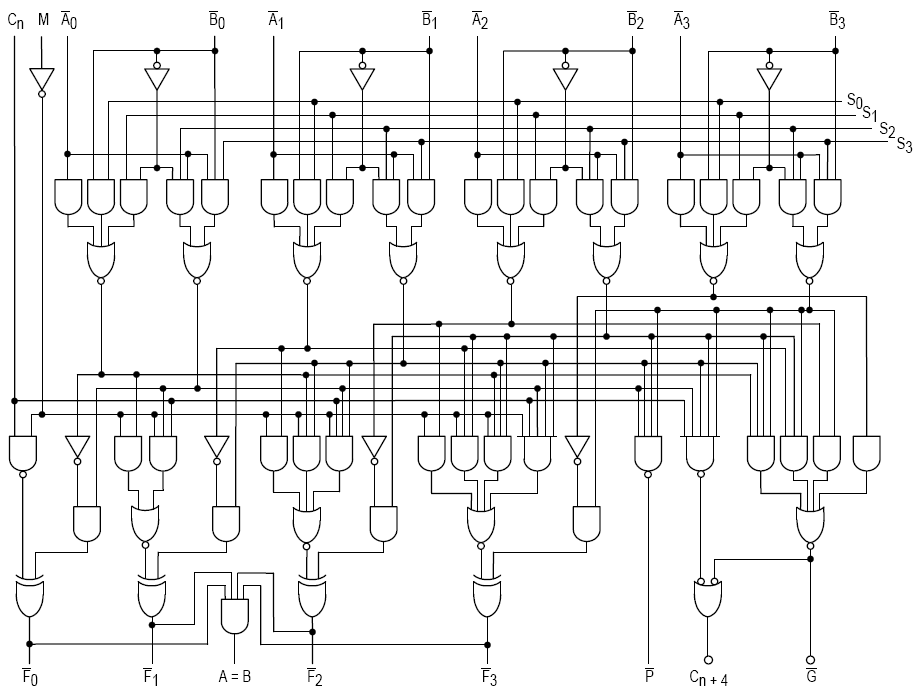
\includegraphics[width=\textwidth]{pictures/ALU.png}
        \caption*{An example of a simple (no joke) four--bit ALU}
    \end{figure}

    \printindex
\end{document}
